% !TeX program = xelatex
% Exactly 20 designed pages, including the opening overview and review checklist.
\documentclass[11pt,a4paper]{article}
\usepackage[left=23mm,right=23mm,top=21mm,bottom=22mm,headheight=15pt]{geometry}
\usepackage{iftex}
\ifPDFTeX
  \usepackage[T1]{fontenc}
  \usepackage[utf8]{inputenc}
  \usepackage{tgpagella,tgheros}
  \usepackage[scale=0.88]{tgcursor}
\else
  \usepackage{fontspec}
  \setmainfont{texgyrepagella-regular.otf}[BoldFont=texgyrepagella-bold.otf,ItalicFont=texgyrepagella-italic.otf,BoldItalicFont=texgyrepagella-bolditalic.otf]
  \setsansfont{texgyreheros-regular.otf}[BoldFont=texgyreheros-bold.otf,ItalicFont=texgyreheros-italic.otf]
  \setmonofont{texgyrecursor-regular.otf}[BoldFont=texgyrecursor-bold.otf,ItalicFont=texgyrecursor-italic.otf,BoldItalicFont=texgyrecursor-bolditalic.otf,Scale=0.88]
\fi
\usepackage{amsmath,amssymb,booktabs,tabularx,array,graphicx,xcolor}
\usepackage{fancyhdr,titlesec,enumitem,listings,needspace,etoolbox,xurl,ragged2e}
\usepackage[protrusion=true,expansion=false]{microtype}
\definecolor{navy}{HTML}{17324D}
\definecolor{teal}{HTML}{277D77}
\definecolor{muted}{HTML}{526371}
\definecolor{wash}{HTML}{F1F4F7}
\definecolor{rulegray}{HTML}{D2DCE3}
\usepackage[unicode,colorlinks=true,linkcolor=navy,urlcolor=teal]{hyperref}
\hypersetup{pdftitle={SafeSliceSQL: The 20-Page Project Guide},pdfauthor={Prepared from the SafeSliceSQL repository},pdfsubject={An accessible complete workflow, worked example, file map, parameters, results and project review}}
\AtBeginDocument{\RaggedRight}
\setlength{\parindent}{0pt}
\setlength{\parskip}{6pt}
\setlength{\emergencystretch}{3em}
\linespread{1.06}
\setlength{\tabcolsep}{4pt}
\renewcommand{\arraystretch}{1.12}
\newcolumntype{P}[1]{>{\RaggedRight\arraybackslash}p{#1}}
\newcolumntype{Y}{>{\RaggedRight\arraybackslash}X}
\setlist[itemize]{leftmargin=1.4em,itemsep=3pt,topsep=4pt}
\setlist[enumerate]{leftmargin=1.7em,itemsep=4pt,topsep=4pt}
\titleformat{\section}{\sffamily\Large\bfseries\color{navy}}{}{0pt}{}
\titleformat{\subsection}{\sffamily\normalsize\bfseries\color{navy}}{}{0pt}{}
\titlespacing*{\section}{0pt}{0pt}{11pt}
\titlespacing*{\subsection}{0pt}{10pt}{4pt}
\pagestyle{fancy}
\fancyhf{}
\fancyhead[L]{\sffamily\small\color{muted}SafeSliceSQL | Understand the project in 20 pages}
\fancyfoot[L]{\sffamily\footnotesize\color{muted}Version 0.1.0 | Source review: 25 November 2026}
\fancyfoot[R]{\sffamily\small\thepage\ / 20}
\renewcommand{\headrulewidth}{0.3pt}
\lstset{basicstyle=\ttfamily\small,keywordstyle=\color{navy}\bfseries,commentstyle=\color{muted},stringstyle=\color{teal},backgroundcolor=\color{wash},frame=single,rulecolor=\color{rulegray},framerule=0.3pt,framesep=6pt,breaklines=true,breakatwhitespace=false,columns=fullflexible,keepspaces=true,showstringspaces=false,tabsize=4,aboveskip=7pt,belowskip=7pt}
\newcounter{guidepage}
\newcommand{\guidepage}[1]{\ifnum\value{guidepage}>0\clearpage\fi\stepcounter{guidepage}\section*{\arabic{guidepage}. #1}\pdfbookmark[0]{\arabic{guidepage}. #1}{guide-\arabic{guidepage}}\label{guide-page-\arabic{guidepage}}}
\newcommand{\remember}[1]{\par\begingroup\setlength{\fboxsep}{8pt}\colorbox{wash}{\parbox{\dimexpr\linewidth-16pt\relax}{\textbf{Keep this idea.} #1}}\endgroup\par}
\newcommand{\owner}[1]{{\small\color{muted}\textbf{Code to open:} #1}\par}
\newcommand{\filemap}[1]{\begingroup\small\par\noindent\begin{tabularx}{\linewidth}{@{}P{.29\linewidth}Y@{}}\toprule\textbf{File} & \textbf{What it does and the important handoff}\\\midrule #1\bottomrule\end{tabularx}\par\endgroup}

\begin{document}

\guidepage{SafeSliceSQL: the complete story}
{\sffamily\Large\color{teal}A practical guide for a first-time reader\par}

Imagine a shop with millions of customer and sale records. A developer wants a small working copy for a test. Selecting unrelated rows can leave a sale whose customer or product is absent. SafeSliceSQL selects records together with the parents they need, stays within a total-row limit, and checks what happens to chosen SQL questions.

The result is a \textbf{separate smaller database}, plus evidence about its size, relationships, query answers and errors. The original is the \textbf{source}; the smaller copy is the \textbf{target}. The project does not automatically hide personal data or guarantee that every original answer remains unchanged.

\subsection*{What to read where}
\par\noindent\begin{tabularx}{\linewidth}{@{}P{.16\linewidth}Y@{}}
\toprule\textbf{Pages} & \textbf{What you will understand}\\\midrule
2--3 & Database basics and the 13-record shop used throughout.\\[4pt]
4--8 & The whole job: input, required parents, selection, copying and safe acceptance.\\[4pt]
9--10 & Worked SQL questions, percentages and integrity checks.\\[4pt]
11--12 & Settings, limits, databases and CSV inputs above 5,000 rows.\\[4pt]
13--16 & Every application module, grouped by its place in the workflow.\\[4pt]
17--18 & Supporting files, tests and actual recorded evidence.\\[4pt]
19--20 & How to run the project and what to explain in a review.\\\bottomrule
\end{tabularx}\par

\subsection*{Which file is ``main''?}
\path{desktop.py} starts the window; \path{cli.py} starts terminal commands. \path{pipeline.py:run_pipeline()} coordinates one complete checked slice. \path{sampler.py} contains the three selection strategies, assisted by \path{dependency_graph.py}. Different files own starting, coordinating and choosing.

\remember{First understand one record's journey. Then use the file map to locate the code. A long list of function signatures is not required to follow the project.}

\textbf{Evidence note.} The shop is fictional and its deliberately chosen copy was executed using project code. It illustrates behavior, not a method-performance benchmark. Saved historical experiments are labelled on page 18. All 20 pages include this opening overview; there is no extra cover or reference appendix.

\guidepage{The essential terms, with an example}
A \textbf{table} stores one kind of thing, such as customers. A \textbf{row} is one record; a \textbf{column} is one kind of value. A Customers table might have the columns customer ID and name, with a row saying ``1, Asha''.

A \textbf{primary key} uniquely identifies a row. Two people can share a name, so an order refers to Customer 1 rather than depending on the name Asha being unique. A \textbf{foreign key} declares that this customer reference must match a real parent record. The order is the child; the customer is its parent.

If Order 101 refers to Customer 1, retaining that order requires Customer 1. Retaining Customer 1 does not require retaining every order the customer ever placed. A child referring to an absent required parent has an \textbf{orphaned reference}.

\subsection*{The words used by the program}
\par\noindent\begin{tabularx}{\linewidth}{@{}P{.25\linewidth}Y@{}}
\toprule\textbf{Term} & \textbf{Read it as}\\\midrule
Schema & The blueprint: tables, columns, types, keys and rules.\\[4pt]
SQL query & A database instruction. The tested questions here use read-only SELECT statements.\\[4pt]
Workload & A list of those questions, usually a .sql file. Statement order gives IDs Q1, Q2 and so on.\\[4pt]
Function & A named piece of work. Its parameters describe inputs; its return value is the result it gives back.\\[4pt]
Object / result type & A structured form containing related fields, such as chosen IDs and their total count.\\[4pt]
Transaction & Related pending database changes. Commit saves them; rollback cancels them.\\[4pt]
Seed & A starting value for repeatable pseudo-random choices; 42 is a default, not a quality score.\\\bottomrule
\end{tabularx}\par

\subsection*{Database versus server versus viewer}
MySQL is the running server that stores and serves databases. Workbench is a viewer/management tool; installing it does not necessarily start a server. SafeSliceSQL's main application uses MySQL 8.x and InnoDB, the transactional table-storage engine.

SQLite is also used for local tests and internal answer comparison. It does not remove the normal desktop CSV flow's MySQL requirement: a CSV is imported into a MySQL source before the smaller MySQL copy is created.

\remember{A function name such as \path{select_rows()} means ``choose record identifiers''. It produces a selection plan; copying and committing are later operations.}

\guidepage{The worked shop: 13 records become six}
Our example has four tables. IDs connect the rows; they are not row counts. Unit prices are ordinary example values, not the copy budget.

\par\noindent\begin{tabularx}{\linewidth}{@{}P{.46\linewidth}P{.46\linewidth}@{}}
\textbf{Customers: 3 rows}\newline 1: Asha\newline 2: Bharat\newline 3: Charu &
\textbf{Products: 3 rows}\newline 10: Notebook, price 50\newline 20: Pen, price 10\newline 30: Bag, price 500\\[10pt]
\textbf{Orders: 3 rows}\newline 101 belongs to Customer 1\newline 102 belongs to Customer 1\newline 103 belongs to Customer 2 &
\textbf{Order lines: 4 rows}\newline Shown below: each line identifies its order, product and quantity.\\
\end{tabularx}\par

\begin{center}\begin{tabular}{rrrr}\toprule
\textbf{Line ID} & \textbf{Order ID} & \textbf{Product ID} & \textbf{Quantity}\\\midrule
1001 & 101 & 10 & 2\\1002 & 101 & 20 & 5\\1003 & 102 & 30 & 1\\1004 & 103 & 20 & 10\\\bottomrule
\end{tabular}\end{center}

There are $3+3+3+4=13$ source rows. At a 50-percent limit, half of 13 is 6.5, rounded down to a cap of \textbf{6 rows}. Every kept customer, product, order and line counts.

Keeping Line 1001 requires that line, Order 101, Customer 1 and Product 10: \textbf{four records}. Adding Line 1002 requires only the new line and Product 20. Its order and customer are already kept. Those \textbf{two new records} fill the remaining slots.

\begin{center}\begin{tabular}{lrrl}\toprule
\textbf{Table} & \textbf{Source} & \textbf{Copy} & \textbf{Kept IDs}\\\midrule
Customers & 3 & 1 & 1\\Products & 3 & 2 & 10, 20\\Orders & 3 & 1 & 101\\Order lines & 4 & 2 & 1001, 1002\\\midrule
\textbf{Total} & \textbf{13} & \textbf{6} & Required parents present\\\bottomrule
\end{tabular}\end{center}

The example keys were deliberately chosen to explain a valid copy. They are not a promise that an automatic method always chooses those keys. The setup and workload SQL, plus checked example results, accompany the source bundle.

\remember{Omitting an unselected record is expected. Omitting a required parent of a retained record is a relationship error.}

\guidepage{The full workflow, from click to result}
\begin{center}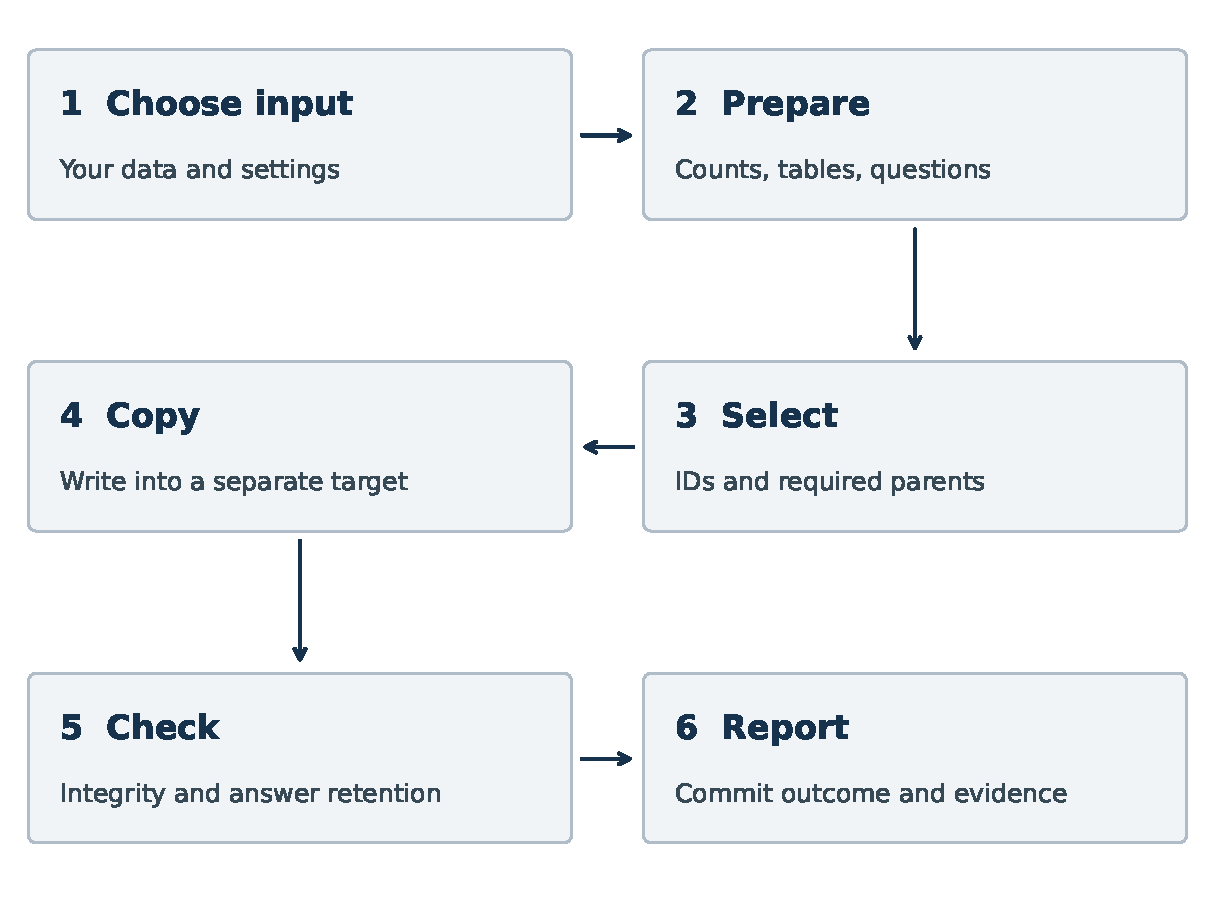
\includegraphics[width=.86\linewidth]{assets/simple-workflow.pdf}\end{center}

\textbf{1. Choose input.} The user selects data, percentage, method, seed and optional custom questions. A checked request records the choices.

\textbf{2. Prepare.} The app previews counts, prepares the source/target, describes table rules, establishes the source view and reads the workload.

\textbf{3. Select.} The chosen method proposes IDs. Required parents are included only when their total added cost fits the cap.

\textbf{4. Copy.} The app writes original values into the separate target in parent-safe order, comparing copied batches with their originals.

\textbf{5. Check.} Before committing the pending row changes, it evaluates questions, validates structure/relationships/budget and applies quality requirements. Rejection rolls back those changes.

\textbf{6. Report.} The app records success or failure, timings and measurements. Results can be viewed, exported and checked again later.

\owner{\path{desktop_service.py} or \path{cli.py} enters the flow; \path{pipeline.py} coordinates a single checked run.}

\guidepage{Prepare the source and the questions}
\subsection*{Two input routes}
For an \textbf{existing MySQL database}, SafeSliceSQL uses the source connection to read its declared types and relationships. It prepares a separate target. Load a downloaded SQL dump using a MySQL client first; the CSV picker does not import .sql dumps.

For \textbf{CSV/folder/XLSX input}, the app creates an owned imported-source schema on the configured target server, imports tables there, then creates a second schema for the smaller output. Generated names look like \path{safeslice_input_<token>} and \path{safeslice_output_<token>}.

File values are preserved as text and receive \path{_safeslice_id} identifiers. CSV empty fields remain empty strings; Excel empty cells can become NULL. Duplicate/blank headers are normalized and mapped in dataset.json. The importer does not infer numeric types or foreign keys between files.

\subsection*{Describe and stabilize the original}
Schema inspection discovers tables, columns, keys and exact counts. A dependency map records parent relationships. A consistent source read view keeps the selected IDs and source answers aligned while the job runs.

A source fingerprint summarizes the observed structure and values, alongside counts. It can detect changed endpoint values even when row counts match. It is evidence about that observed source view, not a history of every external write.

\subsection*{Read the workload}
The lexer recognizes quotes, comments and statement boundaries. The analyzer assigns Q IDs and finds tables, filters, joins, groups and aggregates. Automatic questions demonstrate structure; custom workloads express the questions your test actually needs.

Supported patterns include validated SELECT, WHERE, explicit inner joins, GROUP BY, HAVING and basic COUNT/SUM/MIN/MAX/AVG. Outer/comma joins, subqueries, CTEs, set operations, windows and dynamic/write statements are outside the workload subset. Unsupported questions remain visible with reasons; supported execution failures remain failures.

\owner{\path{dataset_input.py}, \path{schema_analyzer.py}, \path{connection_scope.py}, \path{source_snapshot.py}, \path{sql_lexer.py}, \path{workload_analyzer.py}.}

\guidepage{Required parents and the hard row budget}
A record's \textbf{dependency closure} is the record plus all parents it needs recursively. For the first shop sale line, that means the line, its order, the order's customer and its product.

\begin{center}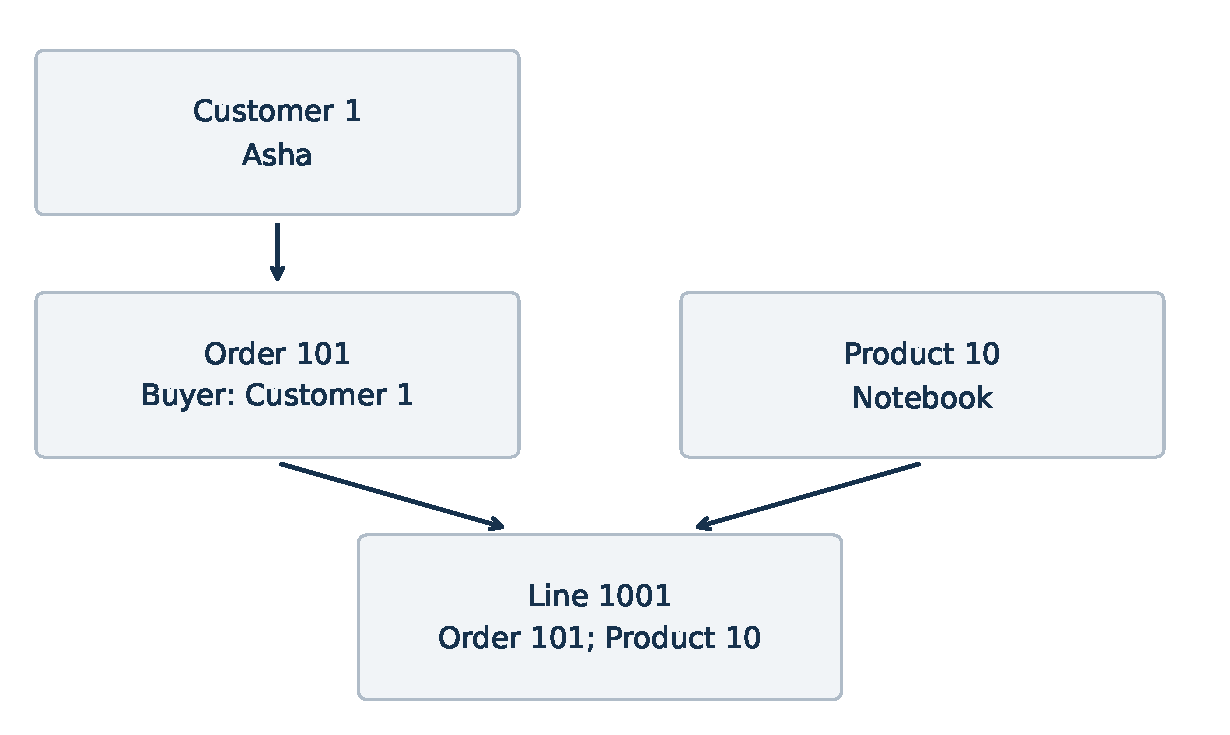
\includegraphics[width=.78\linewidth]{assets/shop-relationships.pdf}\end{center}

The cap counts \textbf{all target rows}, not only the chosen children. For $N$ source rows and percentage $p$, normal CLI/benchmark runs use:
\[
B=\max\left(1,\left\lfloor Np/100\right\rfloor\right).
\]
With 13 source rows and 50 percent, $B=6$. The selector library also permits an explicit zero budget; an empty-input preview displays zero.

\textbf{Incremental cost} counts only records not already selected. Line 1001 costs four slots. Once its parents are kept, Line 1002 costs two. Already-kept parents do not consume another slot when referenced again. A candidate that cannot fit is rejected; unused space is allowed if nothing else fits.

Every supported table needs a declared primary key. Composite primary keys are supported, but composite foreign keys are not. A composite key uses several columns together. Cross-table cycles are unsupported: for example, A requiring B and B requiring A. Same-table references, such as employees pointing to managers, are supported when actual parent chains do not loop.

A nullable foreign key can mean no parent requirement for that value. Keeping a parent does not require every child, so a retained invoice need not retain every original invoice line.

\owner{\path{dependency_graph.py:compute_closure()} returns required IDs; \path{sampler.py} checks their new cost against remaining space.}

\guidepage{The three selection methods}
All three methods share dependency closure, hard-cap enforcement, copying and validation. They differ mainly in the order and priorities used to consider records.

\textbf{Random-repair} considers shuffled candidate IDs. Each accepted child brings its missing required parents, within the same cap. It does not choose a full budget of children and then add unlimited parents.

\textbf{Referential} visits tables in parent-first dependency order with seeded choices within tables. It can spend much of a small budget on parent rows before reaching children useful to a particular query.

\textbf{Workload-aware} first finds real matching IDs from query filters and joins. These small matching sets are called \textbf{witnesses}. Queries get turns, with required IDs prioritized. Remaining space is filled using workload-derived table priorities; every addition still needs feasible parent closure.

\subsection*{The actual priority values}
\par\noindent\begin{tabularx}{\linewidth}{@{}P{.67\linewidth}Y@{}}\toprule
\textbf{Usable query feature} & \textbf{Addition}\\\midrule
Each referenced table & +2.0 to that table\\[3pt]
Each detected join pair & +0.5 to the first table\\[3pt]
Each resolved filter column & +1.0 to its table\\[3pt]
Each resolved grouping column & +1.5 to its table\\[3pt]
Grouping or aggregate present & +1.0 to the first table\\[3pt]
Otherwise unweighted table & Default 1.0\\\bottomrule
\end{tabularx}\par

For the notebook question alone, Order lines and Products each receive 2.0. The join adds 0.5 to Order lines; the product-name filter adds 1.0 to Products. Their priorities are 2.5 and 3.0, while required Orders and Customers must still accompany a retained line.

These are fixed heuristic coefficients, not learned AI parameters. Candidate pooling targets about 1.25 times the budget, with per-table rounding. Suitable integer keys allow indexed guesses; other keys use a streamed seeded sample. Full-source fingerprinting can still be expensive.

\remember{Seed 42 helps reproduce choices on unchanged inputs. It is not a quality score. No method is guaranteed to fill every slot or outperform every other method.}

\guidepage{Copy safely, then accept or reject}
Selection produces a plan of record IDs. Copying is a separate operation. The application first confirms that the actual source and target are different databases. MySQL identity uses the connected server and schema, so a hostname alias cannot make the original safe to overwrite.

Compatible table structures are reproduced or checked. Unrelated target tables, incompatible definitions and pre-existing target triggers are rejected before a refresh. Columns, primary/foreign keys, unique/check constraints and indexes matter; a matching table name alone is insufficient.

\subsection*{Write the records}
Old target rows are deleted child-first. New records are inserted parent-first. In the shop, Customers and Products precede dependent rows, and Order 101 precedes its lines. Supported self-references are ordered at record level. Generated columns are computed by the target.

The default copying batch is 500 rows. Each batch is read back and compared with original values, and the actual total target count is checked. These checks detect problems beyond simply assuming an INSERT succeeded.

\subsection*{Decide before commit}
The pipeline runs workload evaluation, integrity validation and the acceptance policy inside the pending target row transaction. A failed query, structural problem or rejected quality requirement prevents commit and rolls back those row changes.

For the shop, 100-percent eligible query survival passes. A requirement for 60-percent exact answer retention fails because the measured average is 56.67 percent. Structurally valid does not automatically mean good enough for a chosen test.

\subsection*{Know the boundary}
MySQL table/schema creation is not transactional in the same way as ordinary row edits. Handled cleanup removes only structures proven created by the attempt; a hard crash can leave remnants. Cancellation arriving after commit cannot undo the commit.

Participating jobs use a target lock, normally waiting up to five seconds. This coordinates SafeSliceSQL workers, not arbitrary external writers. Use a dedicated target, avoid concurrent schema changes and give source/target accounts appropriate separate permissions.

\owner{\path{pipeline.py}, \path{subset_generator.py}, \path{schema_compatibility.py}, \path{target_lock.py}, \path{validator.py}, \path{acceptance.py}.}

\guidepage{Five questions to test the shop copy}
A workload should be understandable before its percentages are presented. These are the five teaching questions, numbered in statement order. The bundle includes their executable SQL.

\textbf{Q1: which notebook sales remain?} The original and copy both return Line 1001, Notebook, quantity 2.
\begin{lstlisting}[language=SQL]
SELECT l.line_id, p.product_name, l.quantity
FROM order_lines l
JOIN products p ON l.product_id = p.product_id
WHERE p.product_name = 'Notebook';
\end{lstlisting}

\textbf{Q2: which full sale-line records remain?} The original has four; the copy retains two identical records.
\begin{lstlisting}[language=SQL]
SELECT line_id, order_id, product_id, quantity
FROM order_lines;
\end{lstlisting}

\textbf{Q3: which product groups and counts remain?} Notebook changes from 1 to 1 line, Pen from 2 to 1, and Bag is absent in the copy.
\begin{lstlisting}[language=SQL]
SELECT p.product_id, COUNT(*) AS line_count
FROM products p
JOIN order_lines l ON p.product_id = l.product_id
GROUP BY p.product_id;
\end{lstlisting}

\textbf{Q4: how many sale lines are there?} Each database returns one answer row, containing 4 or 2 respectively.
\begin{lstlisting}[language=SQL]
SELECT COUNT(*) AS total_lines FROM order_lines;
\end{lstlisting}

\textbf{Q5: is Customer 999 present?} Neither database has this fictional customer; both answers are empty.
\begin{lstlisting}[language=SQL]
SELECT customer_id, customer_name
FROM customers WHERE customer_id = 999;
\end{lstlisting}

\remember{Q4 survives because it returns a row on both sides, yet its answer changes. Even COUNT on an empty table returns one row containing zero. Survival alone cannot prove answer preservation.}

\guidepage{What the metrics actually mean}
\textbf{Physical row retention} answers ``How much database data was kept?'' Here it is $6/13=46.15\%$. The requested 50 percent is a cap, so rounding to six respects the limit.

\textbf{Query survival} answers ``Does an eligible query still return a nonempty result?'' Q1--Q4 all do, so survival is $4/4=100\%$. Q5 is known source-empty and excluded from that denominator. Supported execution errors remain failed measurements; unknown-source failures are conservatively included as eligible failures.

\begin{center}\begin{tabular}{lrrl}\toprule
\textbf{Query} & \textbf{Source rows} & \textbf{Copy rows} & \textbf{Exact retention}\\\midrule
Q1 & 1 & 1 & 100.00\%\\Q2 & 4 & 2 & 50.00\%\\Q3 & 3 & 2 & 33.33\%\\Q4 & 1 & 1 & 0.00\%\\Q5 & 0 & 0 & 100.00\%\\\bottomrule
\end{tabular}\end{center}

\textbf{Exact result retention} compares complete typed answer tuples, respecting duplicate occurrences. Q3 retains only the unchanged Notebook pair out of three original pairs. Q4's row containing 4 differs from the row containing 2. Empty/empty comparisons get retention 1.0, but do not count as surviving nonempty answers.
\[
\text{Average exact retention}=(1+0.5+1/3+0+1)/5=56.67\%.
\]
\textbf{Key retention} counts distinct safely recognized projected record IDs. \textbf{Aggregate retention} measures identifiable grouping-key coverage when mapping is safe: Q3 keeps two of three product groups, or 66.67 percent, even though Pen's count changed. Both fall back to exact row retention when their mapping is unavailable. The example's overall key/group metric is 63.33 percent.

\subsection*{Integrity is a separate set of checks}
A valid copy needs unique primary keys, zero missing required parents, matching supported structure, an actual count within budget and no failed required checks. Copied batches are value-checked during materialization. Source history may be True, False or unverified; a later count alone cannot prove unchanged content.

Workload means give supported queries equal weight, not weight by answer size. Unsupported SQL is excluded visibly; failed supported evaluations contribute zero. There is no implemented classification F1/FN score or numerical aggregate-error percentage. Group coverage does not measure numeric accuracy.

\guidepage{Parameters, defaults and function values}
\textbf{Desktop defaults:} 10-percent budget, workload-aware method, seed 42, minimum query survival 1.0 and minimum exact retention 0.0. CLI run requires method and budget; CLI/library quality minimums default to zero for compatibility. Required query IDs are initially empty.

The selector library \path{select_rows()} defaults to random-repair, budget 0 and seed 42. That function default differs from the desktop request default. It returns selected IDs and counts; \path{materialize_subset()} later copies them in 500-row chunks. \path{evaluate_workload()} returns per-query and averaged metrics. \path{run_pipeline()} combines the stage outcomes and timings.

\subsection*{Default runtime stop rules}
Environment keys use the prefix \path{SAFESLICE_LIMIT_}; sizes use bytes. Settings must be positive integers.
\par\noindent\begin{tabularx}{\linewidth}{@{}P{.43\linewidth}P{.23\linewidth}Y@{}}\toprule
\textbf{Setting suffix} & \textbf{Default} & \textbf{Meaning}\\\midrule
JOB\_SECONDS & 600 & Whole cooperative job deadline\\[3pt]
STATEMENT\_SECONDS & 30 & Eligible statement/lock setting\\[3pt]
CONNECT\_SECONDS & 10 & MySQL connection timeout\\[3pt]
MAX\_SOURCE\_ROWS & 5,000,000 & All source tables combined\\[3pt]
MAX\_RESULT\_ROWS & 1,000,000 & Rows streamed per query\\[3pt]
MAX\_INPUT\_BYTES & 100 MiB & Input/expanded workbook guard\\[3pt]
MAX\_CELL\_BYTES & 1 MiB & Per imported cell\\[3pt]
MAX\_TEMP\_BYTES & 512 MiB & Temporary comparison database\\[3pt]
MAX\_MEMORY\_BYTES & 1 GiB & Client process RSS guard\\[3pt]
MAX\_TABLES / MAX\_COLUMNS & 100 / 500 & Columns include imported ID\\\bottomrule
\end{tabularx}\par

\textbf{Other useful constants:} candidate multiplier 1.25; decision log limit 1,000; witness prefetch 64; per-query witness cap 1,000; FK prefetch 5,000 keys. File import batches contain 500 rows; record evidence checks use 200-row fetch batches. The source SQL workload contributes the fixed priorities on page 7, not learned coefficients.

Limits are cooperative: memory and cancellation are checked at safe points, so native allocations or a completed commit have their own boundaries. A five-million-row guard is not proof of a successful five-million-row experiment. Restart the desktop after changing its environment settings.

\guidepage{Datasets and databases for useful tests}
Every recommended source below exceeds 5,000 records. For relational databases this means the total across base tables; small lookup tables are normal. CSV counts exclude headers. A smaller target may fall below 5,000.

\par\noindent\begin{tabularx}{\linewidth}{@{}P{.18\linewidth}P{.20\linewidth}Y@{}}\toprule
\textbf{Input} & \textbf{Source rows} & \textbf{First test and purpose}\\\midrule
World & 5,302; 3 tables & 20\% permits 1,060 rows. Follow cities and languages to countries.\\[6pt]
Chinook 1.4.5 & 15,607; 11 tables & 10\% permits 1,560. Test invoice/customer/track chains, playlists and composite keys.\\[6pt]
Employees & 3,919,015; 6 tables & 1\% permits 39,190. Test history/composite keys after smaller inputs. Salaries alone has 2,844,047 rows.\\[6pt]
Diamonds CSV & 53,940; 10 columns & 10\% permits 5,394. Larger text-preserving single-table sampling.\\[6pt]
Taxis CSV & 6,433; 14 columns & 20\% permits 1,286. Timestamp-like strings, payment categories and empty fields.\\\bottomrule
\end{tabularx}\par

\subsection*{Choose matching questions}
Use \path{workloads/testing_world.sql}, \path{testing_chinook.sql} or \path{testing_employees.sql} in the same workloads folder. Each has three targeted questions. The two-query \path{testing_diamonds.sql} and \path{testing_taxis.sql} assume singly imported, original-named CSVs; use dataset.json if names change.

The older \path{workloads/workload.sql} contains eight Employees questions; \path{world_workload.sql} contains six World questions. A workload for one schema will not automatically suit another.

\subsection*{What is local, and what is only recommended?}
This checkout has Diamonds and the smaller Iris/Tips/Penguins/Titanic CSVs, plus ClassicModels and Employees SQL payloads. The four smaller CSVs and ClassicModels are below the larger-source threshold. Local SQLite Employees-like data has only 2,018 source rows; it is not the full upstream Employees database.

README contains download/setup links. Sources are \href{https://dev.mysql.com/doc/index-other.html}{MySQL samples}, \href{https://github.com/lerocha/chinook-database}{Chinook}, \href{https://github.com/datacharmer/test_db}{Employees} and \href{https://github.com/mwaskom/seaborn-data}{Seaborn data}. Downloads are not compatibility certification. Confirm the preview count and run your own selected workload. Downloaded payloads are ignored by Git and absent from fresh clones.

\guidepage{File map: start and prepare}
The next four pages cover all 45 application modules under \texttt{src/safeslicesql/}. Read a file's responsibility before studying its functions. They are cooperating parts of one flow.

\filemap{
\texttt{\_\_init\_\_.py} & Declares version 0.1.0 and re-exports public library operations. Import shortcuts lead to implementations in their owning modules.\\[7pt]
\texttt{desktop.py} & Builds the Tkinter window, collects choices, handles progress/cancellation and opens result views. main() starts the interface.\\[7pt]
\texttt{desktop\_service.py} & Validates CopyRequest; prepares input, writes experiment YAML, runs the shared benchmark and saves CopyOutcome. create\_copy() owns this service lifecycle.\\[7pt]
\texttt{cli.py} & Typer command entrance: inspect, run, validate, benchmark, selftest, scalecheck and jobs. run() enters the same checked core.\\[7pt]
\texttt{demo.py} & Numbered presentation menu. It forwards real choices to existing CLI operations, rather than implementing another sampler.\\[7pt]
\texttt{commands.py} & Wraps CLI work in limits and a job journal. Cancellation exits 130; cooperative limit stops exit 124.\\[7pt]
\texttt{config.py} & Reads private environment settings into separate source/target configuration objects; validates settings and safely constructs connection URLs.\\[7pt]
\texttt{db.py} & Builds/tests connections, quotes identifiers and checks actual source/target identity. An engine manages connections; it is not the stored data.\\[7pt]
\texttt{input\_picker.py} & Opens file/folder dialogs or lists user databases, filtering system schemas. Cancellation does not prepare a dataset.\\[7pt]
\texttt{input\_preview.py} & Reads counts and warnings before writes. preview\_input() shares the import reader; row\_budget() mirrors percentage rounding.\\[7pt]
\texttt{dataset\_input.py} & Streams supported files as text with generated IDs or prepares an existing source. Returns PreparedDataset and dataset.json with mappings.\\[7pt]
\texttt{experiment\_config.py} & Writes method/budget/seed/workload/output/acceptance choices into one YAML instruction file consumed by benchmark.\\[5pt]
}

\subsection*{Follow the first handoff}
A click becomes a CopyRequest, then a PreparedDataset and run.yaml. Settings describe what should happen; the later selection and validation results record what actually happened. Neither configuration file nor an input preview proves that a target was committed.

\guidepage{File map: understand and choose}
These files turn the source blueprint and selected questions into a plan of record IDs. Our shop's first line needs four records; the second adds only two. This reasoning happens before the full records are written.

\filemap{
\texttt{automatic\_workload.py} & Builds structural SELECT examples using discovered names: projections, counts, groups and joins. Large examples are bounded; business intent is not inferred.\\[9pt]
\texttt{schema\_analyzer.py} & inspect\_schema() discovers columns, PKs/FKs and exact counts or reuses same-view counts. Unsupported structures are flagged; failed inspection is not zero rows.\\[9pt]
\texttt{dependency\_graph.py} & DependencyGraph maps parent requirements and order. compute\_closure() resolves actual parents, skips already-paid rows and bounds work by remaining budget.\\[9pt]
\texttt{sql\_lexer.py} & Separates statements/tokens with quote and comment awareness. A semicolon inside a literal must not split the question. Malformed constructs are rejected.\\[9pt]
\texttt{workload\_analyzer.py} & Assigns Q IDs and extracts tables, joins, filters and grouping lineage. It records unsupported syntax and execution status separately.\\[9pt]
\texttt{workload\_candidates.py} & query\_witnesses() projects real matching PKs from original FROM/JOIN/WHERE conditions. Witnesses guide selection but do not solve every aggregate objective.\\[9pt]
\texttt{sampler.py} & select\_rows() dispatches random-repair, referential or workload-aware selection and accepts only feasible incremental closures. Returns SelectionResult with IDs and diagnostics.\\[9pt]
\texttt{types.py} & Defines the shared result forms: schema, closure, selection, generation, validation, queries and benchmark runs. Consistent fields make stages agree on meanings.\\[5pt]
}

\subsection*{What the key functions receive and return}
\texttt{inspect\_schema(engine)} returns the table blueprint. \texttt{analyze\_workload(path, engine)} returns query descriptions. \texttt{select\_rows(..., budget=6, seed=42)} returns chosen identifiers, not copied rows. \texttt{compute\_closure(...)} supplies the complete required set or its incremental missing requirements.

The result carries total selected, added-parent counts, rejected candidates and a bounded decision log. Rejection means an attempted addition did not fit; it is not itself an FK violation. Static priority scores and query witnesses influence which additions are attempted first.

\remember{Structure answers ``What must accompany this record?'' Workload analysis answers ``Which records may help these questions?'' Selection combines those facts under the cap.}

\guidepage{File map: copy and decide}
The central coordinator connects a proposed selection to an accepted database transaction. Read \texttt{pipeline.py}, then the copier and evaluator to understand this boundary.

\filemap{
\texttt{pipeline.py} & run\_pipeline() verifies baseline/read view, takes the target lease, selects IDs, copies and runs the pre-commit checks. Collects success, errors and timings.\\[8pt]
\texttt{subset\_generator.py} & materialize\_subset() checks identity/schema, refreshes rows safely, orders self-references, compares copied batches and invokes checking before commit.\\[8pt]
\texttt{schema\_compatibility.py} & Compares reflected columns, PK/FK definitions, unique/check constraints and indexes by structure. A different constraint name alone is not a structural mismatch.\\[8pt]
\texttt{validator.py} & validate\_subset() checks integrity/budget/source evidence. evaluate\_workload() measures answer, key and grouping retention with explicit failure/empty-result rules.\\[8pt]
\texttt{result\_store.py} & Streams typed answer tuples and occurrence counts into temporary SQLite storage. Exact intersections respect duplicates while avoiding all-results Python memory.\\[8pt]
\texttt{source\_snapshot.py} & Fingerprints observed schema and typed contents, with exact counts. A reused same-view snapshot avoids repeated scans; unchanged counts alone are insufficient.\\[8pt]
\texttt{connection\_scope.py} & Shares one borrowed source transaction among helpers. source\_transaction() keeps selection, copy and comparison on the same repeatable source view.\\[8pt]
\texttt{acceptance.py} & AcceptancePolicy.evaluate() checks measured quality and required Q IDs. It returns pass/fail reasons, not a guarantee the selector can find a better copy.\\[8pt]
\texttt{target\_lock.py} & Serializes participating target writers through a MySQL named lock or SQLite file lock. Busy targets fail after the configured wait.\\[5pt]
}

\subsection*{The important returned forms}
GenerationResult records inserted counts and copying status. ValidationReport records structure, references, cap and source evidence. WorkloadReport records query outcomes and averages. AcceptanceReport records whether chosen quality requirements passed. BenchmarkRunResult joins them with timings and errors.

A copied batch awaiting its checks is not yet an accepted result. Standalone structural validity can permit unverified source history, but the normal pipeline supplies its baseline. Always read the state and error fields with a percentage.

\guidepage{File map: operate, inspect and measure}
\filemap{
\texttt{runtime.py} & Checks cancellation, deadlines and quotas. execution\_context() installs the guard; bounded\_engine() adds appropriate read-only/timeout hooks.\\[5pt]
\texttt{jobs.py} & Atomically journals phases, states and proven schema/server ownership. Recovery marks abandoned jobs interrupted; explicit cleanup checks ownership and age.\\[5pt]
\texttt{security.py} & Resolves environment/file/native-vault credentials and sanitizes public errors. Explicit unreadable secret references fail instead of silently falling back.\\[5pt]
\texttt{logging\_config.py} & Sets console and rotating diagnostic logs, with secret redaction. Diagnostics help locate failures; they are not benchmark evidence alone.\\[5pt]
\texttt{benchmark.py} & Runs every requested method/budget/seed combination through the common pipeline. Saves all attempts; successful measurements form mean/std/count summaries.\\[5pt]
\texttt{reporting.py} & Exports run/per-query CSVs and terminal summaries, preserving checks, acceptance and error evidence.\\[5pt]
\texttt{plots.py} & Draws benchmark-summary charts and handles unavailable measurements without fabricating successful values.\\[5pt]
\texttt{saved\_results.py} & Saves credential-free copy summaries and reopens recorded outcomes with current credentials and ownership/server checks.\\[5pt]
\texttt{copy\_evidence.py} & Reads current copied values and parent facts, beyond a few display samples. collect\_evidence() records verification separately from creation.\\[5pt]
\texttt{record\_browser.py} & Performs parameterized, paged searches and compares original/copied records and parents. Distinguishes kept, omitted, changed and missing-original states.\\[5pt]
\texttt{result\_views.py} & Presents saved outcomes, charts and before/after relationships in Tk windows; it does not implement another sampler.\\[5pt]
\texttt{friendly\_report.py} & Builds escaped, self-contained printable HTML with recorded-time notices. Saved reports are distinct from live inspection.\\[5pt]
\texttt{view\_tasks.py} & Runs read-only tasks in a worker, queues results and invokes UI callbacks through polling. Closing a view requests cancellation.\\[5pt]
\texttt{user\_errors.py} & Explains connection, permission, unavailable-input and limit failures in actionable language with retry/settings options.\\[5pt]
\texttt{synthetic.py} & Generates varied schemas and tests all methods at 10/100 percent, repeatability and full-budget exact results.\\[5pt]
\texttt{scale\_check.py} & Records actual case sizes, wall/CPU time, sampled client RSS and artifact bytes. Labels evidence synthetic, not production certification.\\[3pt]
}

\guidepage{Supporting files, folders and test coverage}
\begingroup\small
\par\noindent\begin{tabularx}{\linewidth}{@{}P{.39\linewidth}Y@{}}\toprule
\textbf{Location} & \textbf{Purpose}\\\midrule
\path{demo.bat}; \path{Terminal Demo.bat} & Launch the desktop or numbered terminal menu from the project environment.\\[5pt]
\path{pyproject.toml} & Version, Python requirement, dependencies/extras, console entry point, pytest and Ruff settings.\\[5pt]
\path{requirements.txt}; pinned demo requirements & General editable installation or the pinned Windows/Python 3.10 demonstration setup.\\[5pt]
\path{.env.example}; private \path{.env} & Public settings template versus your actual private connections/secrets.\\[5pt]
\path{README.md}; \path{docs/} & Setup/download/query instructions; operations and exact supported-scope/metric definitions.\\[5pt]
\path{workloads/}; \path{benchmarks/} & SQL questions and experiment YAML. SQLite example matrix has 27 runs; World matrix has 18.\\[5pt]
\path{examples/demo-orders.csv} & Fictional 20-row interface demo; 25 percent permits five rows.\\[5pt]
\path{datasets/README.md}; manifest & Local download notes, URLs, dimensions, sizes, SHA-256 and archive checks; downloaded payloads remain ignored.\\[5pt]
\path{scripts/seed_sqlite_db.py} & Creates a small Employees-like local SQLite example, not the full upstream data.\\[5pt]
\path{scripts/generate_plots.py} & Calls the plot generator on an existing summary CSV.\\[5pt]
\path{scripts/create_1pct_targets.sql} & Manually creates separate Employees targets for three 1-percent comparisons.\\[5pt]
\path{scripts/least_privilege_mysql.sql} & Administrator-reviewed reader/writer grant example; not executed automatically.\\[5pt]
\path{tests/}; \path{.github/workflows/ci.yml} & Behavior checks and hosted Python/MySQL CI instructions. Configured CI is not proof of a passed hosted run.\\[5pt]
\path{results/}; \path{logs/}; \path{data/} & Saved measurements, diagnostics and ignored local SQLite databases. Check dates and scope.\\[5pt]
\path{build/}; \path{.venv/}; caches & Generated code copies, installed runtime and developer state. Canonical application source is under src.\\\bottomrule
\end{tabularx}\par\endgroup

\subsection*{What the tests establish}
There are 28 behavioral test modules plus shared test support. They cover configuration, schema discovery, parent closure, selectors, SQL parsing, copying/rollback, result metrics, imports, UI services, reports, ownership and resource controls. Regression tests check that previously fixed edge cases stay fixed.

Database-marked tests need their configured service. A non-database run does not demonstrate fresh MySQL integration results. Source controls, tests and reports together support a review; an old build folder or cache does not.

\guidepage{What results can you actually claim?}
\textbf{Teaching example, executed for explanation.} The deliberately chosen shop copy keeps 6 of 13 rows, fits its six-row cap, has zero missing parents and passes structural checks. Its eligible query survival is 100 percent, average exact retention 56.67 percent and average key/group metric 63.33 percent. It is not a method-performance trial.

\textbf{Verification of the inspected source.} The earlier check recorded \textbf{368 non-database tests passed}, 32 database-marked cases deselected, lint passed, and \textbf{30 SQLite generated checks passed}. This document condenses the explanation; it does not relabel those checks as a new MySQL run.

\subsection*{A saved 20-row demo}
A recorded copy kept five rows at a 25-percent cap. All three eligible queries survived, while exact-retention fractions were 0.25, 0 and 0.25. Their mean is 16.67 percent. The count answer changed from 20 to 5, illustrating why survival differs from unchanged answers.

\subsection*{Historical World comparison: 10-percent budget}
\begin{center}\begin{tabular}{lrr}\toprule
\textbf{Method} & \textbf{Mean survival} & \textbf{Mean exact retention}\\\midrule
Random-repair & 100.00\% & 15.03\%\\
Referential & 83.33\% & 12.53\%\\
Workload-aware & 83.33\% & 12.60\%\\\bottomrule
\end{tabular}\end{center}
Source: \path{results/raw/all_benchmark_runs.csv}, artifact date 2 November 2026. It contains 18 saved successful runs over budgets 10/20/30 and seeds 42/123; the table shows two-seed means at 10 percent. It predates the inspected source, lacks an embedded source commit and uses older timing fields. It does not establish current universal superiority.

\subsection*{Saved MySQL scale evidence}
\path{results/scale/6893236af2c9/evidence.json} records five generated shapes and 30 checks per scale sample, with zero failures. The larger sample's largest case contains 40,463 total rows; it records about 426.58 seconds wall time and 262.73 MiB sampled peak client RSS. It excludes MySQL server resource totals and explicitly is not production certification.

\remember{Read attempted, successful and failed counts beside means. Summary averages use successful measured runs; one observation has no sample standard deviation. A quick mean from few successes does not prove reliability.}

\guidepage{Run it and verify a useful copy}
\subsection*{Launch the desktop}
MySQL must be running and the project environment/settings installed. From PowerShell:
\begin{lstlisting}[language={}]
cd C:\Users\saivi\Projects\SafeSliceSQL
.\demo.bat
\end{lstlisting}
If the window does not open, run the console interpreter to see the error:
\begin{lstlisting}[language={}]
.\.venv\Scripts\python.exe -m safeslicesql.desktop
\end{lstlisting}

\textbf{CSV test.} Choose Diamonds, set 10 percent, select \path{workloads/testing_diamonds.sql} in Options and create the copy. Expect no more than 5,394 rows. Imported values are text, so its queries use category filters and generated IDs.

\textbf{Relational test.} Import World or Chinook into MySQL first, choose MySQL database and its matching testing workload. Inspect the preview, fix a seed and set explicit quality requirements. Required parents count toward the percentage.

\subsection*{A World relationship question}
\begin{lstlisting}[language=SQL]
SELECT cl.CountryCode, cl.Language, co.Name
FROM countrylanguage cl
JOIN country co ON cl.CountryCode = co.Code
WHERE cl.IsOfficial = 'T';
\end{lstlisting}
After a successful run, open Verify my copy, compare a retained record with its original, follow a parent and export the report. Standalone CLI validation should receive the experiment's actual cap:
\begin{lstlisting}[language={}]
safeslice validate --source world --target YOUR_COPY --budget-limit 1060 --workload workloads/testing_world.sql
\end{lstlisting}
Without that cap, standalone validation defaults to full current source size. It also cannot reconstruct earlier source history without a baseline.

\textbf{Manual orphan check in a MySQL client:} the following must return zero on source and copy. Keep it outside workload SQL because LEFT JOIN is unsupported by the workload subset.
\begin{lstlisting}[language=SQL]
SELECT COUNT(*) AS orphan_cities
FROM city ci LEFT JOIN country co
  ON ci.CountryCode = co.Code
WHERE co.Code IS NULL;
\end{lstlisting}

\guidepage{What to highlight in your project review}
\subsection*{A clear opening}
``SafeSliceSQL creates a smaller working database under a hard total-row budget. A selected child brings its required parent records, so a sale is not left without its order, customer or product. I then check the copy and measure how many chosen query answers remain.''

\subsection*{Show the project in this order}
\begin{enumerate}
\item \textbf{Problem and example:} explain why Line 1001 costs four records and Line 1002 adds only two. This makes parent closure and the budget concrete.
\item \textbf{Implementation:} show pipeline.py as coordinator, sampler.py as selector, dependency\_graph.py as relationship reasoning, subset\_generator.py as copier and validator.py as checker.
\item \textbf{Demonstration:} show exact input counts, settings and actual copied count. Inspect a retained row and its parent, not just a success banner.
\item \textbf{Metrics:} explain physical rows, query survival and exact answer retention separately. Use the changed COUNT result to demonstrate the difference.
\item \textbf{Comparison and evidence:} use matched workloads/budgets/seeds, report failures as well as means, and label saved results and synthetic tests accurately.
\end{enumerate}

\subsection*{Answers you should be ready to give}
\textbf{Why three methods?} Two baselines help test whether workload priorities improve a chosen task under the same closure, budget and evaluation rules.

\textbf{Is the proposed method learned or optimal?} It is a seeded heuristic with fixed coefficients and actual query witnesses. It does not prove the best possible subset and need not beat every baseline.

\textbf{What is guaranteed by relationships?} Retained supported children have required parents. Child rows, groups and numeric totals can still be lost or changed, so workload usefulness needs its own measurement and quality gate.

\textbf{What happens on rejection?} Pending target row changes roll back before commit. MySQL DDL/hard-crash cleanup has separate boundaries; a post-commit cancel cannot undo saved changes.

\textbf{What are the limits?} Restricted schema/SQL scope, no automatic PII masking and no production-capacity certification. Larger representative schemas, more seeds and application-specific questions are sensible next experiments.

\remember{The central result is a checked smaller copy with measured tradeoffs. Explain what was preserved, what was lost, how it was tested and which claims the evidence actually supports.}

\end{document}
